\chapter{Introduction}
\textit{by Olaf Kolditz and Hua Shao}

Motivation part
\begin{itemize}
  \item THMC processes are important ...
  \item application areas ...
\end{itemize}

%-------------------------------------------------------------------------
\section{Scope of this book}

The intention of this book is multifold:
\begin{itemize}
  \item Theoretical background of THMC processes in porous media (chapter \ref{cha:theory})
  \item DDB provides a collection of test cases which are used for benchmarking the GeoSys code development.
  \item The benchmark collection can be a starting point for own numerical exercises and applications.
  \item How to develop and set-up bechmarks for numerical code.
\end{itemize}

%-------------------------------------------------------------------------
\section{Application areas}

The coupling phenomena of thermal (T), hydraulic (H), and mechanical (M) processes are important for the analysis of deep geosystems under high temperature, pressure and stress conditions. Application areas of THM coupled models are e.g. geothermal energy utilization, nuclear waste deposition, and carbon dioxide storage in the deep subsurface.

The following sildes illustrate that the understanding of THM processes including chemical reactions (C processes) is important to a large variety geotechnical and geothermal applications. The mechanical basics are exactly the same for these applications. Different is simply

\begin{itemize}
	\item the geological environment, i.e. different rock types, crystalline rocks, volcanic rocks, sandstones, clay, bentonite, ...
	\item the geofluids, i.e. water, brines, vapour, methane, carbon dioxid ...
	\item the thermodynamic conditions, i.e. temperature, stress, pressure, salinity, ...
\end{itemize}

Fig. \ref{fig:apl1} shows the application area: Nuclear waste deposition.
There are several concepts concerning the subsurface deposition of hazardeous waste, i.e. using crystalline, salt and volcanic formations as host rock. These concepts include different buffer systems for the waste isolation, i.e. an geotechnical barrier. THMC modeling (including chemistry) is required for the long-term analysis of possible processes which might result in a release of contaminants from the repository. In that case it is important to know, how long will it take until the contaminants can return into the surface biosphere.

Fig. \ref{fig:apl2} illustrates the application area: Carbon Capture Storage (CCS). The idea is to capture the \CO2 from the power plants, liquify it and inject it into the subsurface for long-term storage. Two basic concepts for appropriate geological systems are under proof now: depleted gas reservoirs and deep saline aquifers. After many years of operation many fromer gas reservoirs are depleted. These resrvoir are in an underpressurized status and can take up large volumes of fluids. Keeping the reversoir underpressurized and the imperviuos cap rocks are part of the storage concepts. 
THMC modeling is required in order to calculate the possible fluid storage capacity and to better understand the highly coupled processes in the \CO2 injection area as well as their consequences for the storage concept.

Fig. \ref{fig:apl3} depicts the application area: Geothermal energy, which is one of the alternative future energy resources under consideration. So-called shallow and deep geothermal systems are distinguished. Shallow systems are already commercially used e.g. for heating purposes. Deep geothermal reservoirs can be used for electric power production as high temperatures up to 200 C can be produced. 
THMC modeling is required to design those geothermal power plants, e.g. in order to optimize production efficiency and reservoir lifetime. The significant cooling of the reservoir due to fluid reinjection gives raise to thermo-mechanical effects which needs to be controlled in order to avoid reservoir damage.

\newpage
.
\vspace{6.5cm}
\begin{figure}[htb!]
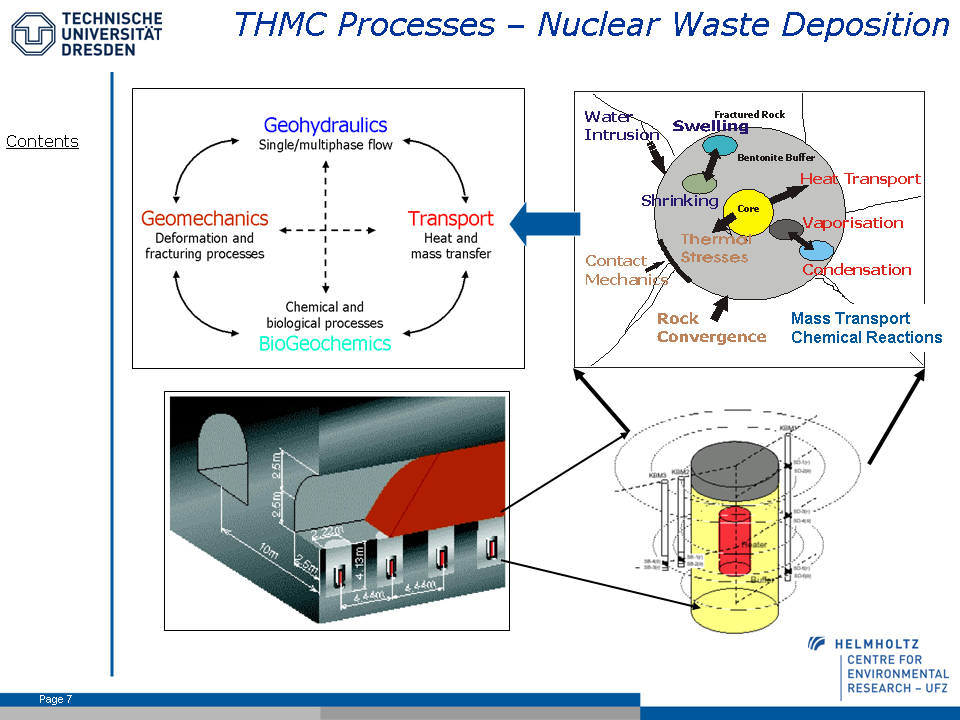
\includegraphics[width=0.07\textwidth]{figures/THMC-Lecture_1.png}
\caption{Application to nuclear waste deposition}
\label{fig:apl1}
\end{figure}
.
\vspace{7.5cm}
\begin{figure}[htb!]
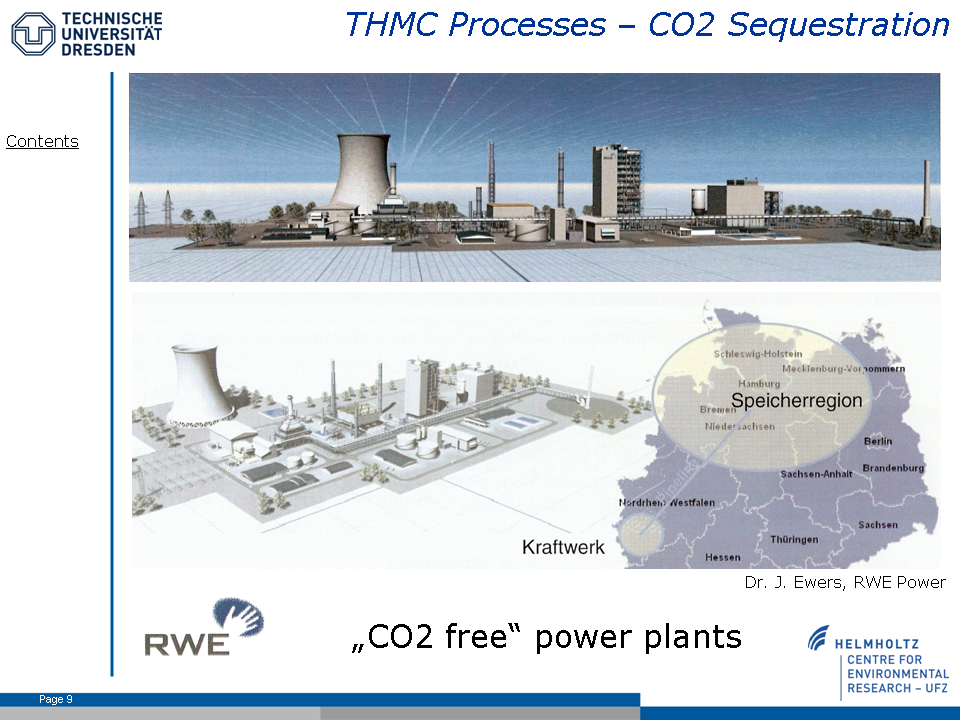
\includegraphics[width=0.07\textwidth]{figures/THMC-Lecture_2.png}
\caption{Application to Carbon-Capture-Storage (CCS) technology}
\label{fig:apl2}
\end{figure}
.
\newpage
.
\vspace{6.5cm}
\begin{figure}[htb!]
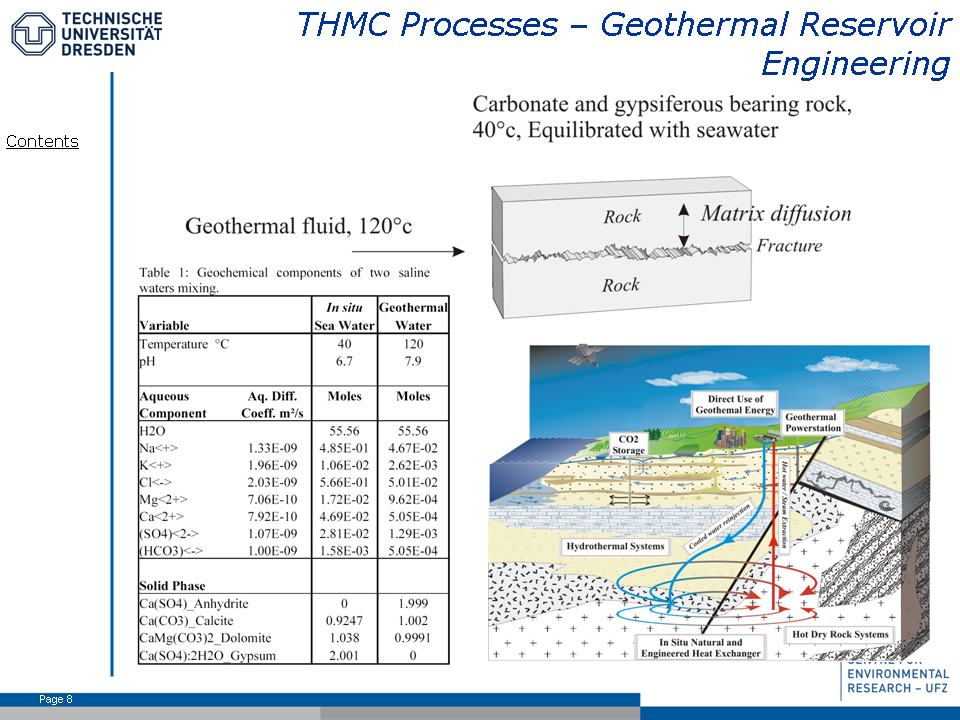
\includegraphics[width=0.07\textwidth]{figures/THMC-Lecture_3.png}
\caption{Application to geothermal reservoir engineering}
\label{fig:apl3}
\end{figure}

%-------------------------------------------------------------------------
\section{Future work}

\begin{itemize}
  \item ...
\end{itemize}

